\documentclass[a4paper, 11pt]{article}
\usepackage{amsmath}
\usepackage{graphicx}
\usepackage{geometry}
\usepackage{listings}
\usepackage{color}
\usepackage{cite}

\definecolor{dkgreen}{rgb}{0,0.6,0}
\definecolor{gray}{rgb}{0.5,0.5,0.5}
\definecolor{mauve}{rgb}{0.58,0,0.82}
\lstset{frame=shadowbox,
    language=Python,
    aboveskip=3mm,
    belowskip=3mm,
    showstringspaces=false,
    columns=flexible,
    basicstyle={\small\ttfamily},
    numbers=left,
    numberstyle=\tiny\color{gray},
    keywordstyle=\color{blue},
    commentstyle=\color{dkgreen},
    stringstyle=\color{mauve},
    breaklines=true,
    breakatwhitespace=true,
    tabsize=3
}
\usepackage[colorlinks,linkcolor=red]{hyperref}
\geometry{scale=0.8}

\title{	
\normalfont \normalsize
\textsc{School of Data and Computer Science, Sun Yat-sen University} \\ [25pt] %textsc small capital letters
\rule{\textwidth}{0.5pt} \\[0.4cm] % Thin top horizontal rule
\huge 15-Puzzle Problem (IDA*)\\ % The assignment title
\rule{\textwidth}{2pt} \\[0.5cm] % Thick bottom horizontal rule
\author{17341203 Yixin Zhang}
\date{\normalsize\today}
}

\begin{document}
\maketitle
\tableofcontents
\newpage

\section{IDA* Algorithm}
\subsection{Description}
Iterative deepening A* (IDA*) was first described by Richard Korf in 1985, which is a graph traversal and path search algorithm that can find the shortest path between a designated start node and any member of a set of goal nodes in a weighted graph. 

It is a variant of \textbf{iterative deepening depth-first search} that borrows the idea to use a heuristic function to evaluate the remaining cost to get to the goal from the \textbf{A* search algorithm}. 

Since it is a depth-first search algorithm, its memory usage is lower than in A*, but unlike ordinary iterative deepening search, it concentrates on exploring the most promising nodes and thus does not go to the same depth everywhere in the search tree. 

\textbf{Iterative-deepening-A* works as follows:} at each iteration, perform a depth-first search, cutting off a branch when its total cost $f(n)=g(n)+h(n)$ exceeds a given threshold. This threshold starts at the estimate of the cost at the initial state, and increases for each iteration of the algorithm. At each iteration, the threshold used for the next iteration is the minimum cost of all values that exceeded the current threshold.


\subsection{Pseudocode}
\begin{figure}[ht]
\centering
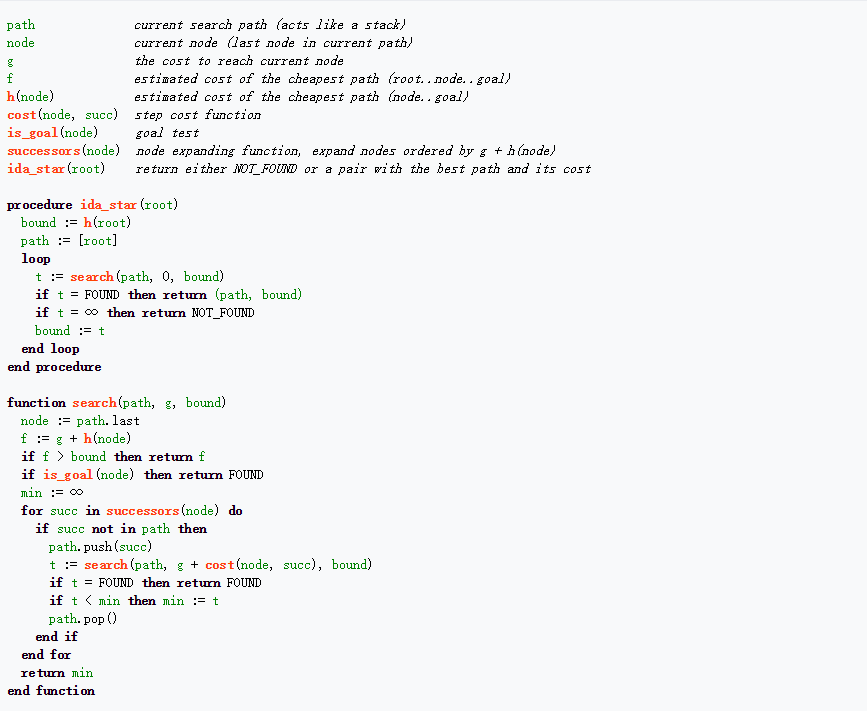
\includegraphics[width=17.3cm]{assets/code}
\end{figure}
\section{Tasks}



\begin{itemize}
	\item Please solve 15-Puzzle problem by using IDA* (Python or C++). You can use one of the two commonly used heuristic functions: h1 = the number of misplaced tiles. h2 = the sum of the distances of the tiles from their goal positions. 
	\item Here are 4 test cases for you to verify your algorithm correctness. You can also play this game (\texttt{15puzzle.zip}) for more information.
	\begin{figure}[ht]
	\centering
	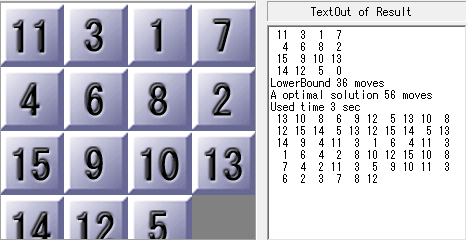
\includegraphics[width=8cm]{assets/case1}
	\quad
	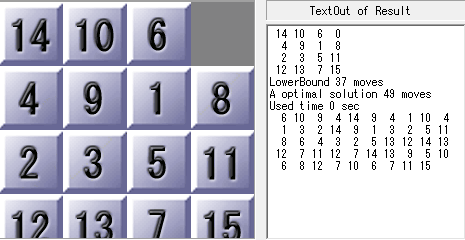
\includegraphics[width=8cm]{assets/case2}
	\\
	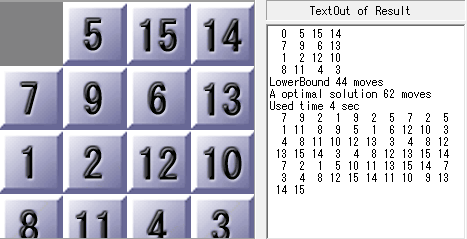
\includegraphics[width=8cm]{assets/case3}
	\quad
	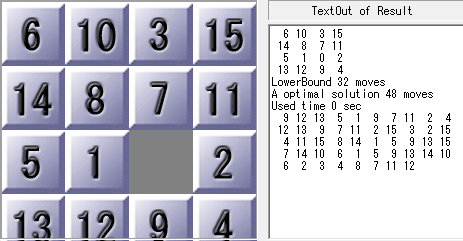
\includegraphics[width=8cm]{assets/case4}
	
	\end{figure}
	\item Please send \texttt{E02\_YourNumber.pdf} to \texttt{ai\_201901@foxmail.com}, you can certainly use \texttt{E02\_15puzzle.tex} as the \LaTeX template.
\end{itemize}


\section{Implementation}

\subsection{Overview}
Thanks to the succinct syntax of Python, we can easily rewrite the pseudocode in section 1.2 into Python code. The program contains only one file `main.py'. Each function's doc string explains what it does.

\subsection{Code}
\begin{lstlisting}[title=main.py]
# -*- coding: utf-8 -*-
import numpy as np
import datetime

def isGoal(node):
    """
    Test if the given node (state) is the goal.
    """
    goal = np.append(range(1, sidelen * sidelen), 0).reshape(sidelen, sidelen)
    return (node == goal).all()


def h1(node):
    """
    Heuristic function 1: using the number of misplaced tiles.
    """
    goal = np.append(range(1, sidelen * sidelen), 0).reshape(sidelen, sidelen)
    return sidelen * sidelen - np.count_nonzero(goal == node) 


def h2(node):
    """
    Heuristic function 2: using Manhattan distance.
    """
    target = {}
    count = 1
    for i in range(sidelen):
        for j in range(sidelen):
            target[count] = (i, j)
            count += 1
    target[0] = (sidelen-1, sidelen-1)

    total_distance = 0
    for i in range(sidelen):
        for j in range(sidelen):
            val = node[i, j]
            total_distance += abs(i - target[val][0]) + abs(j - target[val][1])
    return total_distance


def ida_star(root):
    """
    Do IDA* algorithm from node `root`.
    """
    bound = h2(root)  # initial bound
    path = [root]
    while True:
        ret = search(path, 0, bound)
        if ret == True:
            return path
        if ret == float('inf'):
            return False
        else:
            bound = ret


def search(path, g, bound):
    """
    Do the DFS.
    """
    node = path[-1]  # current node is the last node in the path
    f = g + h2(node)  # heuristic function
    if f > bound:
        return f
    if isGoal(node):
        return True

    temp = np.where(node == 0)  # find the blank
    blank = (temp[0][0], temp[1][0])  # blank's position

    succs = []
    moves = [(0, -1), (0, 1), (-1, 0), (1, 0)]  # up, down, left, right
    for move in moves:
        next_blank = tuple(np.sum([blank, move], axis=0))
        if next_blank[0]>=0 and next_blank[0]<sidelen and next_blank[1]>=0 and next_blank[1]<sidelen:
            succ = node.copy()
            succ[blank], succ[next_blank] = succ[next_blank], succ[blank]
            succs.append(succ)

    _min = float('inf')
    succs.sort(key=lambda x: h2(x))
    for succ in succs:
        if not any((succ == x).all() for x in path):  # special syntax
            path.append(succ)
            t = search(path, g+1, bound)
            if t == True:
                return True
            if t < _min:
                _min = t
            path.pop()
    return _min


def makeActions(path):
    """
    Constuct a list containing numbers to be moved in each step.
    """
    if path == False:
        raise ValueError('No solution!')

    actions = []
    for i, node in enumerate(path[1:]):
        temp = np.where(node == 0)  # find the blank
        blank = (temp[0][0], temp[1][0])  # blank's position
        actions.append(path[i][blank])
    return actions


if __name__ == '__main__':
    print('***STARTING***', datetime.datetime.now().strftime('%Y.%m.%d %H:%M:%S'))

    filename = 'mytest.txt'
    puzzle = np.loadtxt(filename, dtype=np.uint8)  # number 0 indicates the blank
    sidelen = len(puzzle)  # side length of puzzle
    result = makeActions(ida_star(puzzle))
    print(result)
    print('Length:', len(result))

    print('***Finished***', datetime.datetime.now().strftime('%Y.%m.%d %H:%M:%S'))

\end{lstlisting}


\section{Results}
The test cases given above are all too big for my Python code to solve, so I've made my own test cases. Four tests are presented below, each with my solution and a solution from `15puzzle Optimal Solver'\cite{puzzlesolver}.

	\begin{figure}[ht]
	\centering
	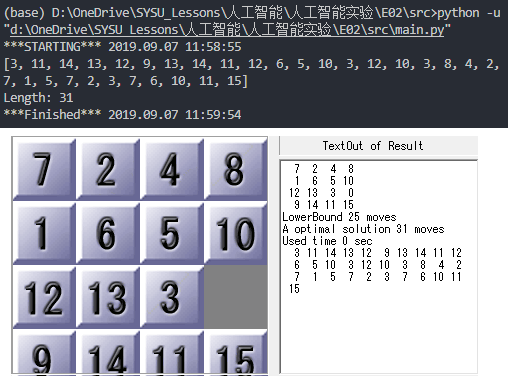
\includegraphics[width=8cm]{assets/mytest1}
	\quad
	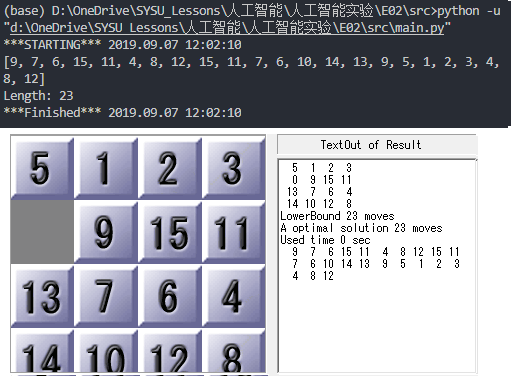
\includegraphics[width=8cm]{assets/mytest2}
	\\
	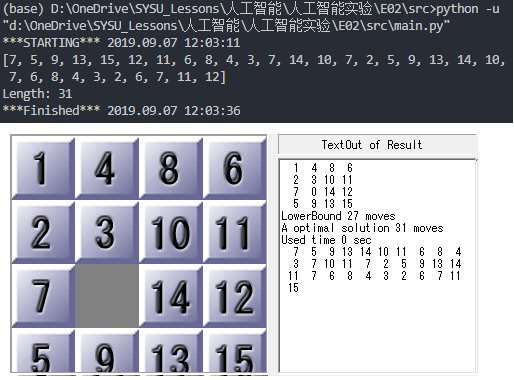
\includegraphics[width=8cm]{assets/mytest3}
	\quad
	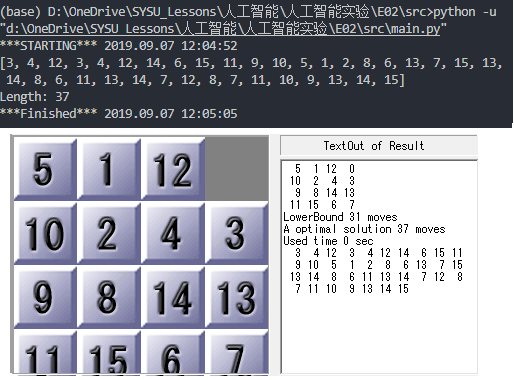
\includegraphics[width=8cm]{assets/mytest4}
	
	\end{figure}

\begin{figure}
\centering
%%\includegraphics[width=15cm]{result.png}
\end{figure}


\section{Discussion}
The IDA* algorithm itself is not hard to understand, but the code implementation progress requires some efforts. I've met several obstacles while writing Python code. The numpy arrays are unhashable, so they cannot be used as keys in Python dictionaries. Due to the special performance on logical operators (such as `and', `or', `not') used on numpy arrays, the syntax must be taken care of -- in most cases, keywords like `all' and `any' should be used.

At last, I found that my Python code turns out to be very slow when the number of steps exceed 40. I think it is because not only Python always runs more slowly than C++, but the heuristic function using Manhattan distance is not good enough. For further study, a heuristic function using `walking distance' might be considered.


\begin{thebibliography}{9}
\bibitem{puzzlesolver} 
15puzzle Optimal solver, \texttt{http://www.ic-net.or.jp/home/takaken/e/15pz/}
\end{thebibliography}
\end{document} 